\section{The Heston Model}

\subsection{Model Description}

\begin{align}
    \label{eq:heston_model_price}
    \mathrm{d}S_t &= \mu S_t\mathrm{d}t + \sqrt{v_t}S_t\mathrm{d}W_t^S \\
    \label{eq:heston_model_log_price}
    \mathrm{d}X_t = \mathrm{d}\log(S_t) &= \left(\mu-\frac{1}{2}v_t\right)\mathrm{d}t + \sqrt{v_t}\mathrm{d}W_t^S \\
    \label{eq:heston_model_variance}
    \mathrm{d}v_t &= \kappa(\theta-v_t)\mathrm{d}t + \sigma\sqrt{v_t}\mathrm{d}W_t^v \\
    \label{eq:heston_model_correlation}
    \mathbb{E}(\mathrm{d}W_t^S\mathrm{d}W_t^v) &= \rho\mathrm{d}t
\end{align}

\subsection{Characteristic Function and Density of the Heston Model}
- Hat eine Zufallsvariable $X$ eine Dichte $f(x)$, so kann man die charakteristische Funktion $\phi(t)$ von $X$ berechnen durch
\begin{align}
    \phi(t) = \mathbb{E}(\exp(\mathrm{i}tX)) = \int_{-\infty}^{\infty} e^{\mathrm{i}tx}f(x)\mathrm{d}x \notag
\end{align}
- Die charakteristische Funktion für eine Zufallsvariable existiert immer, auch wenn die Dichte nicht existiert. Hat man die charakteristische Function, so kann man die Dichte durch die inverse Fourier-Transformation berechnen
\begin{align}
    f(x) = \frac{1}{2\pi}\int_{-\infty}^{\infty} e^{-\mathrm{i}tx}\phi(t)\mathrm{d}t \notag
\end{align}
- Gatheral (2011) hat die charakteristische Funktion des Heston-Modells berechnet
\begin{align}
    \phi(t) = \exp(A + B + C) \notag
\end{align}
mit
\begin{align}
    A &= \mu\cdot\tau\cdot t\cdot\mathrm{i} \notag \\
    d &= \sqrt{(\rho\sigma\mathrm{i}t - \kappa)^2 - \sigma^2(-\mathrm{i}t - t^2)} \notag \\
    g &= \frac{\kappa - \rho\sigma\mathrm{i}t - d}{\kappa - \rho\sigma\mathrm{i}t + d} \notag \\
    B &= \frac{\theta\kappa}{\sigma^2}\left(\tau(\kappa - \rho\sigma\mathrm{i}t - d) - 2\log\left[\frac{1-g\exp(-d\tau)}{1-g}\right]\right) \notag \\
    \gamma &= \frac{2\kappa\theta}{\sigma^2} \notag \\
    C &= \log\left(\left[\frac{2\kappa}{\sigma^2}\right]^{\gamma}\cdot \left\lbrace \frac{2\kappa}{\sigma^2} - \frac{\kappa - \rho\sigma\mathrm{i}t - d}{\sigma^2}\cdot\frac{1 - \exp(-d\tau)}{1-g\exp(-d\tau)} \right\rbrace^{-\gamma}\right) \notag
\end{align}
und $\tau = T-t$ als Zeithorizont.
- Eine simple inverse Fourier-Transformation ist nicht sinnvoll, da es zu numerischen Instabilitäten an den Rändern kommt (siehe \ref{fig:ifft_comparison}). Bei der simplen Methode wird $\phi(t)$ zentiert und $f(x)$ mit der Schrittweite $\Delta t$ normiert um korrekte Amplituden zu erhalten. Die andere Methode verwendet eine Randkorrektur, was die Rekonstruktion der Dichte verbessert. Zudem werden die Ergebnisse durch eine kubische Spline-Interpolation geglättet.

\begin{figure}[h]
    \centering
    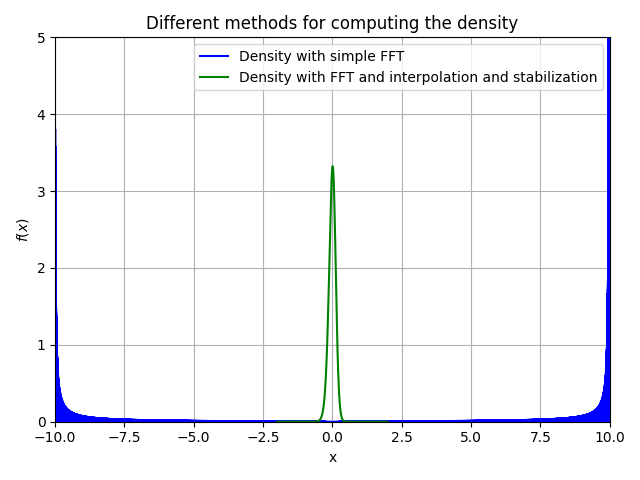
\includegraphics[width=0.8\textwidth]{img/different_ifft_methods.png}
    \caption{Comparison of different methods for the inverse Fourier transformation of the characteristic function of the Heston model ($\mu=0$, $\kappa=3$, $\theta=0.19$, $\sigma=0.4$, $\rho=-0.7$, $\tau=\frac{1}{12}$). Grid points: $N=2^{15}$}
    \label{fig:ifft_comparison}
\end{figure}

\subsection{Simulating the Heston Model}